\documentclass[12pt]{beamer}

\usepackage{amssymb,amsmath,mathtext}
\usepackage{indentfirst,amsfonts}
\usepackage{makecell,multirow,longtable}
\usepackage{graphicx}
\usepackage{color}
\usepackage{verbatim}


\graphicspath{{graphs/}}

\usepackage[english,russian]{babel}
\usepackage[T2A]{fontenc}
\usepackage[utf8]{inputenc}

\setbeamertemplate{navigation symbols}{}

\usetheme{Boadilla}

\beamersetuncovermixins{\opaqueness<1>{30}}{\opaqueness<2->{25}}

\setbeamerfont{frametitle}{series=\bfseries}
\setbeamerfont{block title}{series=\bfseries}

\begin{document}
\title{Нейросетевой синтез текстур с трендами}
\author{Будакян Я.\,С. \\ Научный руководитель к.т.н., доц. Грачев Е.\,А.}
\date{2017 г.} 

\maketitle

\begin{frame}\frametitle{Введение}
	Цель работы состоит в построении процедуры синтеза изображений среды, которые будут содержать в себе тренд. Под текстурой с трендом понимается изображение, в котором есть изменение некоторой характеристики вдоль одного из направлений. Такими характеристиками, например, могут быть изменение интенсивности появления частиц среды или изменение пористости среды. \\
	\begin{figure}
		\centering{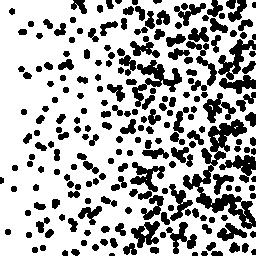
\includegraphics[width=0.3\linewidth]{trend-sample}}
		\caption{Пример текстуры с трендом интенсивности частиц.}
		\label{trend-example}
	\end{figure}
\end{frame}

\begin{frame}\frametitle{Математическая постановка}
	Рассмотрим многомерное пространство $X$, содержащее множество всех изображений $x$: $X = \{x\}$. Обучающая выборка изображений с трендами $D = \{x_i\}$ задает в этом пространстве вероятностное распределение $P_X$, такое, что точки, соответствующие изображениям из выборки, имеют высокую вероятность, а остальные - низкую. Тогда с математической точки зрения задача синтеза текстуры с трендом сводится к синтезу случайного изображения $x'$, принадлежащего распределению, близкому к задаваемому обучающей выборкой:
	$$ P_{X'} \approx P_X, \quad x' \sim X'$$
\end{frame}

\begin{frame}\frametitle{Математическая постановка}
	Для упрощения задачи, сузим множество изображений с трендами до множества изображений, удовлетворяющих следующим ограничениям:
	\begin{itemize}
		\item Это монохромные изображения 256 x 256 пикселей
		\item Изменяющимся свойством является интенсивность появления частиц $\lambda$
		\item Тренд является линейным и направлен вдоль оси изображения $z_1$: 
		$ \lambda = \lambda_0 + kz_1 $
	\end{itemize}
\end{frame}

\begin{frame}\frametitle{Существующие подходы к синтезу}
	Есть несколько подходов к решению задач подобного рода:
	\begin{itemize}
		\item 'Классический' статистический подход
		\item Базовый нейросетевой подход
		\item Генеративные состязательные сети (Generative Adversarial Networks - GAN)
	\end{itemize}
\end{frame}

\begin{frame}\frametitle{'Классический' статистический подход}
	\begin{itemize}
		\item Вводится параметризированное семейство распределений вероятности $P_{\theta}(x)$
		\item Параметры $\theta$ находятся из обучающей выборки:
		$$ \mathcal{L}_{\theta}(D) = \prod_{x \in D} P_{\theta}(x) $$
		$$ \theta^{*} = \underset{\theta}{\arg\max} \mathcal{L}_{\theta}(D)$$
		\item Генерируется объект(изображение) из $ P_{\theta^{*}}$
	\end{itemize}
	Этот подход приводит к проблемам:
	\begin{itemize}
		\item Пространство $\theta$ может быть огромной размерности
		\item Известной параметрической модели распределения может вообще не существовать
	\end{itemize}
	Простой пример - синтез человеческих лиц: с помощью классического подхода эта задача не была решена с хорошим качеством.
\end{frame}

\begin{frame}\frametitle{Базовый нейросетевой подход}
	\begin{itemize}
		\item Вводится параметризированное семейство распределений вероятности $P_{\theta}(x)$
		\begin{itemize}
			\item Вводятся скрытые переменные $V$ и функция(нейросеть) для получения $x$ из $V$ (фактически, классификация, развернутая в другую сторону)
		\end{itemize}
		\item Определяются параметры распределения (т.е. обучение нейросети)
		\item Генерируется объект(изображение) из $ P_{\theta^{*}}$
	\end{itemize}
	Этот подход возможен, однако на практике трудноосуществим или не приводит к хорошему качеству генерации.
\end{frame}

\begin{frame}\frametitle{GAN}
	Архитектура GAN была придумана в 2014 году специально для решения задачи генерации объектов из сложных распределений. \\
	\begin{itemize}
		\item Переформулируем изначальную задачу нахождения такой процеруды генерирования $X'$, чтобы $ P_{X'} \approx P_X$:
		$$ \rho(P_{X'}, P_X) \longrightarrow \underset{P_{X'}}{\min} $$
		\item Введем параметризированную процедуру генерации:
		$$ X' = g_{\theta}(\cdot) $$
		\item Переформулируем:
		$$ \rho(P_{X'}, P_X) \longrightarrow \underset{P_{X'}}{\min} $$
		$$ \rho(g_{\theta}(\cdot), P_X) \longrightarrow \underset{g_{\theta}(\cdot)}{\min} $$
		$$ \rho(g_{\theta}(\cdot), P_X) \longrightarrow \underset{\theta}{\min} $$
	\end{itemize}
	
\end{frame}

\begin{frame}\frametitle{GAN}
	Возникает вопрос: что использовать в качестве метрики похожести двух распределений $\rho$, где одно из распределений задано обучающей выборкой.
	\begin{itemize}
		\item В качестве такой метрики можно использовать функцию потерь обученного классификатора, потому что естественно предположить, что чем чаще ошибается обученный классификатор, тем больше одно распределение похоже на другое:
		$$ \rho(P_{X'}, P_X) \longrightarrow \min \Leftrightarrow L \longrightarrow \max, $$
		где $L$ - функция потерь обученного классификатора.
	\end{itemize}
\end{frame}

\begin{frame}\frametitle{GAN}
	\begin{itemize}
		\item Введем две нейросети:
		\begin{itemize}
			\item $d_{\zeta}(x)$ - классификатор для измерения расстояния, \textbf{дискриминатор}
			\item $g_{\theta}(x)$ - сеть, трансформирующая шум в $X'$, \textbf{генератор}
		\end{itemize}
	\end{itemize}
	Суть использования двух сетей состоит в том, что они обучаются совместно, конкурируя друг с другом: генератор пытается имитировать целевое распределение, а дискриминатор пытается классифицировать поступающие от генератора и из обучающей выборки изображения на 2 класса: реальные (из изначального распределения $P_X$) и ложные (из $P_{X'}$, т.е. произведенные генератором).
\end{frame}

\begin{frame}{GAN}
	\begin{itemize}
		\item Функция потерь обученного классификатора:
		$$ L^*(\theta) = \underset{\zeta}{\min} L(\zeta, \theta) $$
		\item Соответственно,
		$$ \underset{\zeta}{\min} L(\zeta, \theta) \longrightarrow \underset{\theta}{\max} $$
		$$ \theta^* = \underset{\theta}{\arg\max} \left[ \underset{\zeta}{\min} L(\zeta, \theta) \right] $$
		 \item Определим оптимальный дискриминатор:
		 $$ d^*_{\theta} = d_{\zeta^*(\theta)} $$
		 $$ \zeta^*(\theta) =  \underset{\zeta}{\arg\min} L(\zeta, \theta)$$
	\end{itemize}
\end{frame}

\begin{frame}\frametitle{Обучение GAN}
	Таким образом, процесс обучения сети типа GAN принимает следующий вид:
	\begin{columns}
		\column{0.5\linewidth}
			\begin{itemize}
				\item Обучаем дискриминатор при фиксированном генераторе
				\item Обучаем генератор при фиксированном дискриминаторе
				\item Повторяем до сходимости параметров обеих моделей
			\end{itemize}
		\column{0.5\linewidth}
			\begin{figure}
				\centering{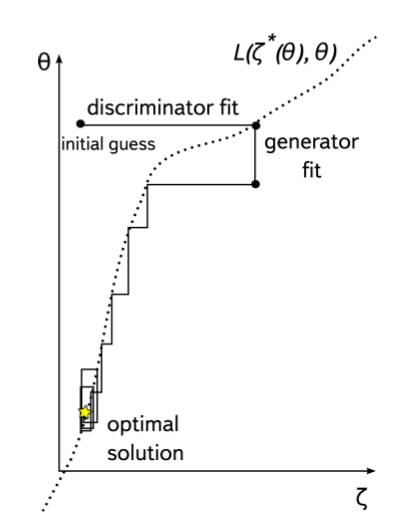
\includegraphics[width=0.65\linewidth]{gan-training}}
				\caption{Схематическое изображение процесса обучения GAN.}
				\label{gan-train}
			\end{figure}
	\end{columns}
\end{frame}

\begin{frame}\frametitle{pix2pix GAN}
	Для решения задачи было попробовано применить модификацию GAN-сети под названием "pix2pix GAN". Ее отличие от схемы GAN, введенной ранее, состоит в том, что вместо шума на вход генератору приходят другие изображения, на которых он основывается при синтезе.
	\begin{columns}
		\column{0.5\linewidth}
			\begin{figure}
				\centering{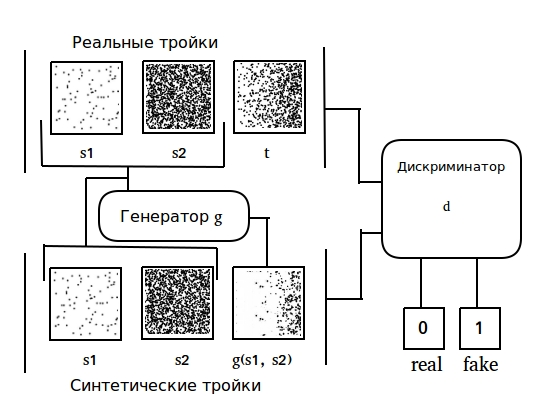
\includegraphics[width=0.85\linewidth]{p2p}}
				\caption{Схематическое устройство сети pix2pix GAN.}
				\label{p2p}
			\end{figure}
		\column{0.5\linewidth}
			\begin{figure}
				\centering{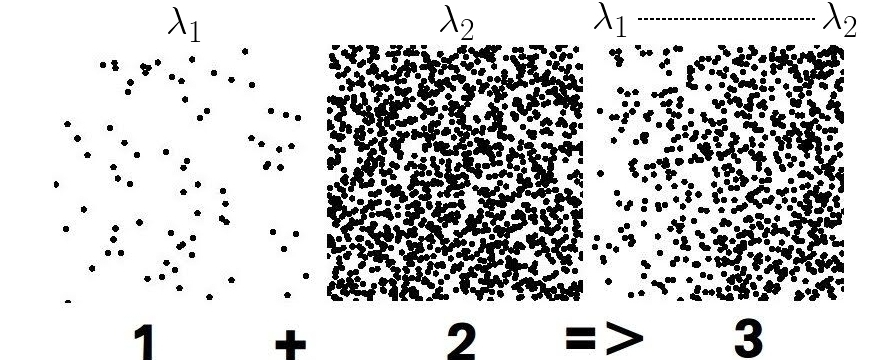
\includegraphics[width=1.0\linewidth]{p2p-gen}}
				\caption{Вход и желаемый выход нейросети-генератора.}
				\label{p2p-gen}
			\end{figure}
	\end{columns}
\end{frame}

\begin{frame}\frametitle{pix2pix GAN}
	\begin{figure}
		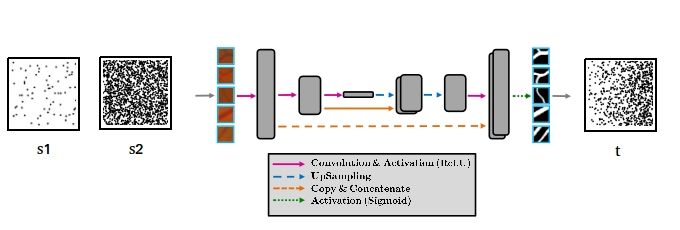
\includegraphics[width=1.0\linewidth]{unet-scheme}
		\caption{Схематическое изображение нейросети-генератора.}
	\end{figure}
\end{frame}

\begin{frame}\frametitle{Критерий качества}
	После обучения генератора, необходимо проверить, что сгенерированные им изображения действительно имеют искомые характеристики. Было решено использовать среднюю плотность черных пикселей в некотором окне, и проходить этим окном по изображению:
	\begin{columns}
		\column{0.5\linewidth}
			$$\xi_k = \frac{1}{H w}{\sum_{i=k}^{k+w} \sum_{j=0}^{H}\left| \frac{x(i, j) - 255}{255} \right|}, $$$$k = \overline{1, W - w + 1} $$
		\column{0.4\linewidth}
			\begin{figure}
				\centering{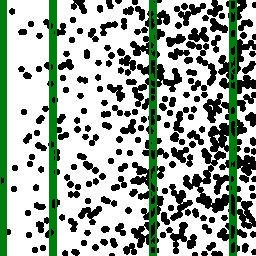
\includegraphics[width=0.7\linewidth]{metrics}}
				\caption{Прохождение окном по изображению}
			\end{figure}
	\end{columns}
\end{frame}

\begin{frame}\frametitle{Критерий качества}
	Построив график $\xi(k)$ можно увидеть, как меняется плотность пикселей и прослеживается ли тренд. В качестве метрики можно взять среднеквадратичную ошибку:
	$$ \xi = \frac{1}{W-w}\sum_{k=1}^{W-w+1} (\xi_k - \xi_{0k})^2,$$
	где $\xi_{0k}$ - $\xi_k$, усредненное по примерам из обучающей выборки.
\end{frame}

\begin{frame}\frametitle{Результаты}
	Было проведено обучение нейросети описанной архитектуры при различных гиперпараметрах (в частности, количестве фильтров на первом сверточном слое). Обучающей выборкой был массив из 3500 троек изображений.
	\begin{figure}
		\begin{columns}
			\column{0.33\linewidth}
				\begin{minipage}{1\linewidth}
					\centering{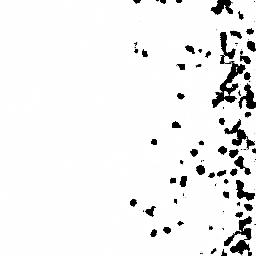
\includegraphics[width=0.5\linewidth]{nf8} \\ nf8}
				\end{minipage}
				\vfill
				\begin{minipage}{1\linewidth}
					\centering{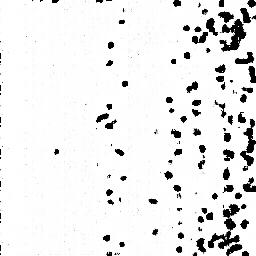
\includegraphics[width=0.5\linewidth]{nf16} \\ nf16}
				\end{minipage}
			\column{0.33\linewidth}
				\begin{minipage}{1\linewidth}
					\centering{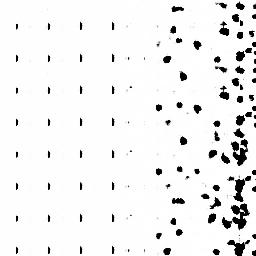
\includegraphics[width=0.5\linewidth]{nf16_woUnet} \\ nf16-woUnet}
				\end{minipage}
				\vfill
				\begin{minipage}{1\linewidth}
					\centering{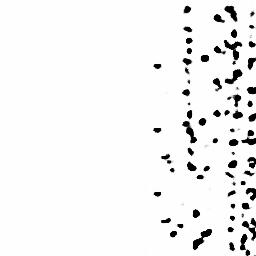
\includegraphics[width=0.5\linewidth]{nf16_3x3_woUnet} \\ nf16-3x3-woUnet}
				\end{minipage}
			\column{0.33\linewidth}
				\begin{minipage}{1\linewidth}
					\centering{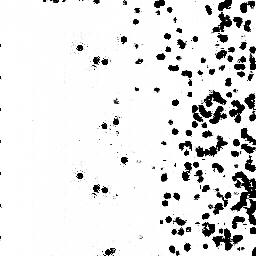
\includegraphics[width=0.5\linewidth]{nf32} \\ nf32}
				\end{minipage}
				\vfill
				\begin{minipage}{1\linewidth}
					\centering{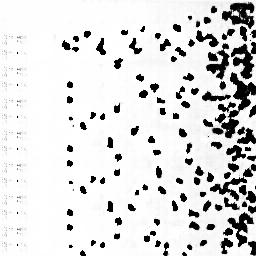
\includegraphics[width=0.5\linewidth]{nf32_woUnet} \\ nf32-woUnet}
				\end{minipage}
		\end{columns}
		\caption{Примеры сгенерированных текстур.}
	\end{figure}
\end{frame}

\begin{frame}\frametitle{Результаты}
	Для сгенерированных наборов текстур получились следующие результаты:
	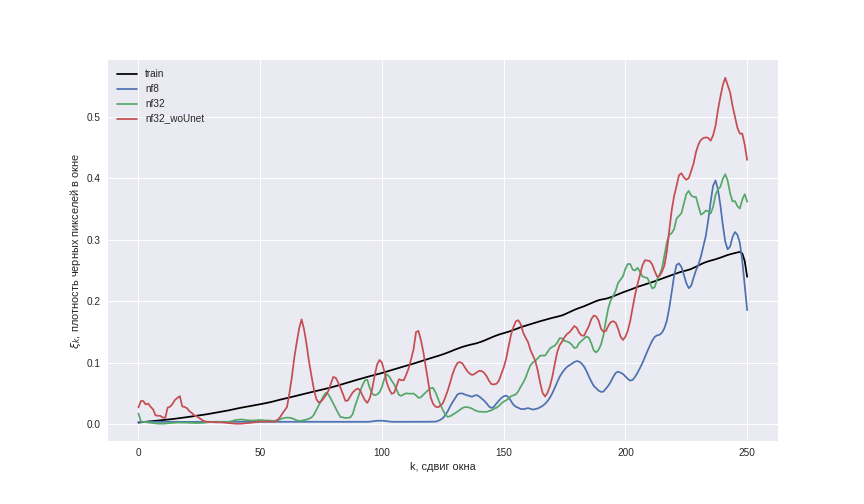
\includegraphics[width=0.9\linewidth,height=0.3\textwidth]{tr_1}
	\begin{table}[h]
		\begin{tabular}{|c|c|}
			\hline
			Сеть & Метрика \\
			\hline
			nf8 & 0.00825\\
			\hline
			nf32 & 0.00549\\
			\hline
			nf32-woUnet & 0.00688\\
			\hline
		\end{tabular}
		\caption{Значения введенной метрики для разных сетей (меньше - лучше)}
	\end{table}
\end{frame}

\begin{frame}\frametitle{Результаты}
	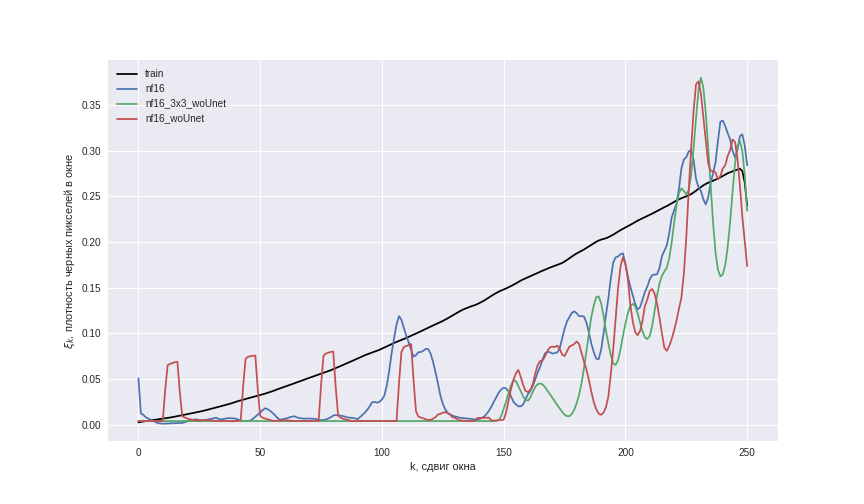
\includegraphics[width=0.9\linewidth,height=0.3\textwidth]{tr_2}
	\begin{table}[h]
		\begin{tabular}{|c|c|}
			\hline
			Сеть & Метрика \\
			\hline
			nf16 & 0.00606\\
			\hline
			nf16-woUnet & 0.00881\\
			\hline
			nf16-3x3-woUnet & 0.01034\\
			\hline
		\end{tabular}
		\caption{Значения введенной метрики для разных сетей (меньше - лучше)}
	\end{table}
\end{frame}

\begin{frame}\frametitle{Заключение}
	В работе было:
	\begin{itemize}
		\item Исследовано применение архитектуры GAN для синтеза текстур с трендами
		\item Получены результаты синтеза при нескольких наборах гиперпараметров сети
		\item Проведено измерение качества генерации для каждого из наборов, используя введенную метрику
	\end{itemize}
	Полученные результаты показывают, что в принципе нейросеть способна уловить тренд и воспроизвести его, однако на данный момент качество генерации относительно невысоко. Необходимо провести дальнешее исследование оптимальных гиперпараметров, и, возможно, увеличить объем обучающей выборки. Также можно провести аналогичные эксперименты с другими архитектурами генераторов.
\end{frame}

\begin{frame}\frametitle{Список использованных источников}
	\begin{thebibliography}{99}
		\bibitem{Voron-ML}  Воронцов К. В., "Математические методы обучения по прецедентам (теория обучения машин)".
		\bibitem{GAN} Ian J. Goodfellow, Jean Pouget-Abadie, Mehdi Mirza, Bign Xu, David Warde-Farley, Sherjil Ozair, Aaron Courville, Yoshua Bengio, "Generative Adversarial Nets" // arXiv: 1406.2661 [stat.ML], 2014
		\bibitem{GAN-2} Goodfellow, Ian, et al. "Generative adversarial nets. Advances in neural information processing systems". 2014
		\bibitem{p2p} Pedro Costa, Adrian Galdran, Maria Inês Meyer, Michael David Abràmoff, Meindert Niemeijer, Ana Maria Mendonça, Aurélio Campilho, "Towards Adversarial Retinal Image Synthesis" // arXiv: 1701.08974 [cs.CV], 2017	
	\end{thebibliography}
\end{frame}

\end{document}